\newlength{\bibsep}
\documentclass[nonatbib,5p,a4paper]{elsarticle}  % 5p for two columns, 1p for 1 column (this is specific for the elsearticle)
\usepackage[italian,norsk,nynorsk]{babel}        % Language
\usepackage[DatePublished]{Code/NTNU-lab}        % remove [DatePublished] to remove dates
\usepackage{csquotes}                            % Must be loaded when babel is loaded to avoid error.
% Use this file to write code that you do not want in the .sty file, but has to be in the preamble (before \begin{document}).
% Writing in this file in stead of in the preamble will keep the main file more organised and tidy.


%                       Nomenclatures
%_______________________________________________________________
\usepackage[intoc]{nomencl}
\makenomenclature

\renewcommand{\nomname}{%
% Title
%----------------
List of Symbols
%----------------
}
\renewcommand{\nompreamble}{%
% Description
%----------------
The next list describes several symbols that will be later used within the body of the document
%----------------
}
% This code creates the groups
\renewcommand\nomgroup[1]{%
  \item[\bfseries
  \ifstrequal{#1}{A}{Physics constants}{%
  \ifstrequal{#1}{B}{Mathematical constants}{%
  \ifstrequal{#1}{C}{Other symbols}{}}}%
]}
% This will add the units
\newcommand{\nomunit}[1]{%
\renewcommand{\nomentryend}{\\#1}}
%................................................................

                            % Write all preamble code in this file to keep it organised and tidy.

\addbibresource{Bibliography/Sources.bib}        % Selects the Bibliography file.


\begin{document}
\selectlanguage{italian}                         % Sets the language of the document.

%%%%%%%%%%%%%%%%%%%%%%%%%%%%%%%%%%%%%%%%

\begin{frontmatter}
%
% Title:
%------------------------------------
\title{Circuiti 3}
%
% Authors:
%------------------------------------
% List an author with name ' Firstname Middlename Lastname ' like this:
% F. M. Lastname
\author{L. Trombetta} 
\author{A. Turturiello}
\author{F. Venturoli}
%
% Date:
%------------------------------------
%
\newdate{dateName}{19}{06}{2022} % edit the date here, ' dateName ' has to match on these two lines.
\renewcommand*{\today}{\MonthYearDateFormat\displaydate{dateName}} 
% Options for displaying date: \MonthYearDateFormat,  \DayMonthYearDateFormat or \YearDateFormat
%
% Abstract:
%------------------------------------

\NameOfAbstract{Abstract}
 % Change abstract title here. If you write in Norwegian, write 'Sammendrag' (nb) or 'Samandrag' (nn)
\begin{abstract}
% Delete the text and write your abstract here:
%------------------------------------

Lo scopo dell'esperienza è stato quello di studiare i circuiti RC, RL e RLC attraverso la nozione di impedenza e, quindi, di funzione di trasferimento in corrente impulsata a onda sinusoidale e delle diverse componenti circuitali.

\end{abstract}
%
\end{frontmatter}
%
%
% Table of contents:
%------------------------------------
% If the report is very long for some reason (over 4 or 5 pages), use a table of contents.
% Uncomment everything below the line ---- to get table of contents (ctrl + /) (the / on numberpad):
%-------------
%
% \ 
 \vspace{1cm}

 \begin{minipage}{\textwidth}
     \tableofcontents
 \end{minipage}
 \clearpage
%% Prints a list of symbols. You can create/ change the categories in the preamble.tex file. 
% Learn more about nomenclature: https://www.overleaf.com/learn/latex/Nomenclatures

\nomenclature[A, 02]{\(c\)}{\href{https://physics.nist.gov/cgi-bin/cuu/Value?c}
{Speed of light in a vacuum}
\nomunit{\SI{299792458}{\meter\per\second}}}
\nomenclature[A, 03]{\(h\)}{\href{https://physics.nist.gov/cgi-bin/cuu/Value?h}
{Planck constant}
\nomunit{\SI[group-digits=false]{6.62607015e-34}{\joule\per\hertz}}}
\nomenclature[A, 01]{\(G\)}{\href{https://physics.nist.gov/cgi-bin/cuu/Value?bg}
{Gravitational constant} 
\nomunit{\SI[group-digits=false]{6.67430e-11}{\meter\cubed\per\kilogram\per\second\squared}}}
\nomenclature[B, 03]{\(\mathbb{R}\)}{Real numbers}
\nomenclature[B, 02]{\(\pi\)}{Pi}
\nomenclature[B, 01]{\(e\)}{Euler's constant}
\nomenclature[C]{\(V\)}{Constant volume}
\nomenclature[C]{\(\rho\)}{Friction index}
\printnomenclature

                 % List of symbols, can be useful
\section{Introduzione e descrizione dell'apparato sperimentale}
Per condurre l'esperienza ci siamo serviti di una Breadboard dotata di due boccole e di una griglia di fori in cui inserire i refori. La griglia è caratterizzata dalla presenza di quattro colonne indicate con i simboli "+" e "-", ciascuna equipotenziale, e altre venti colonne equipotenziali riga per riga, indicate con delle lettere. Lo strumento ci ha permesso di realizzare i circuiti su cui abbiamo condotto le diverse misure. Le componenti di circuito di cui ci siamo serviti sono state le resistenze, di cui abbiamo ricavato i valori tramite un \textit{tool online}\footnote{ https://www.digikey.it/it/resources/conversion-calculators/conversion-calculator-resistor-color-code}, diodi di silicio e un partitore resistivo, composto da boccole e da interruttori in grado di modificare la resistenza dello strumento.
Abbiamo fatto uso di due multimetri, strumenti in grado di misurare diverse grandezze, nel nostro caso utilizzati per determinare la differenza di potenziale tra due punti del circuito e l'intensità di corrente.
Infine, abbiamo collegato un generatore che fornisse corrente ai circuiti, attraverso il controllo della sua differenza di potenziale.

\begin{figure}[h!]
    \centering
    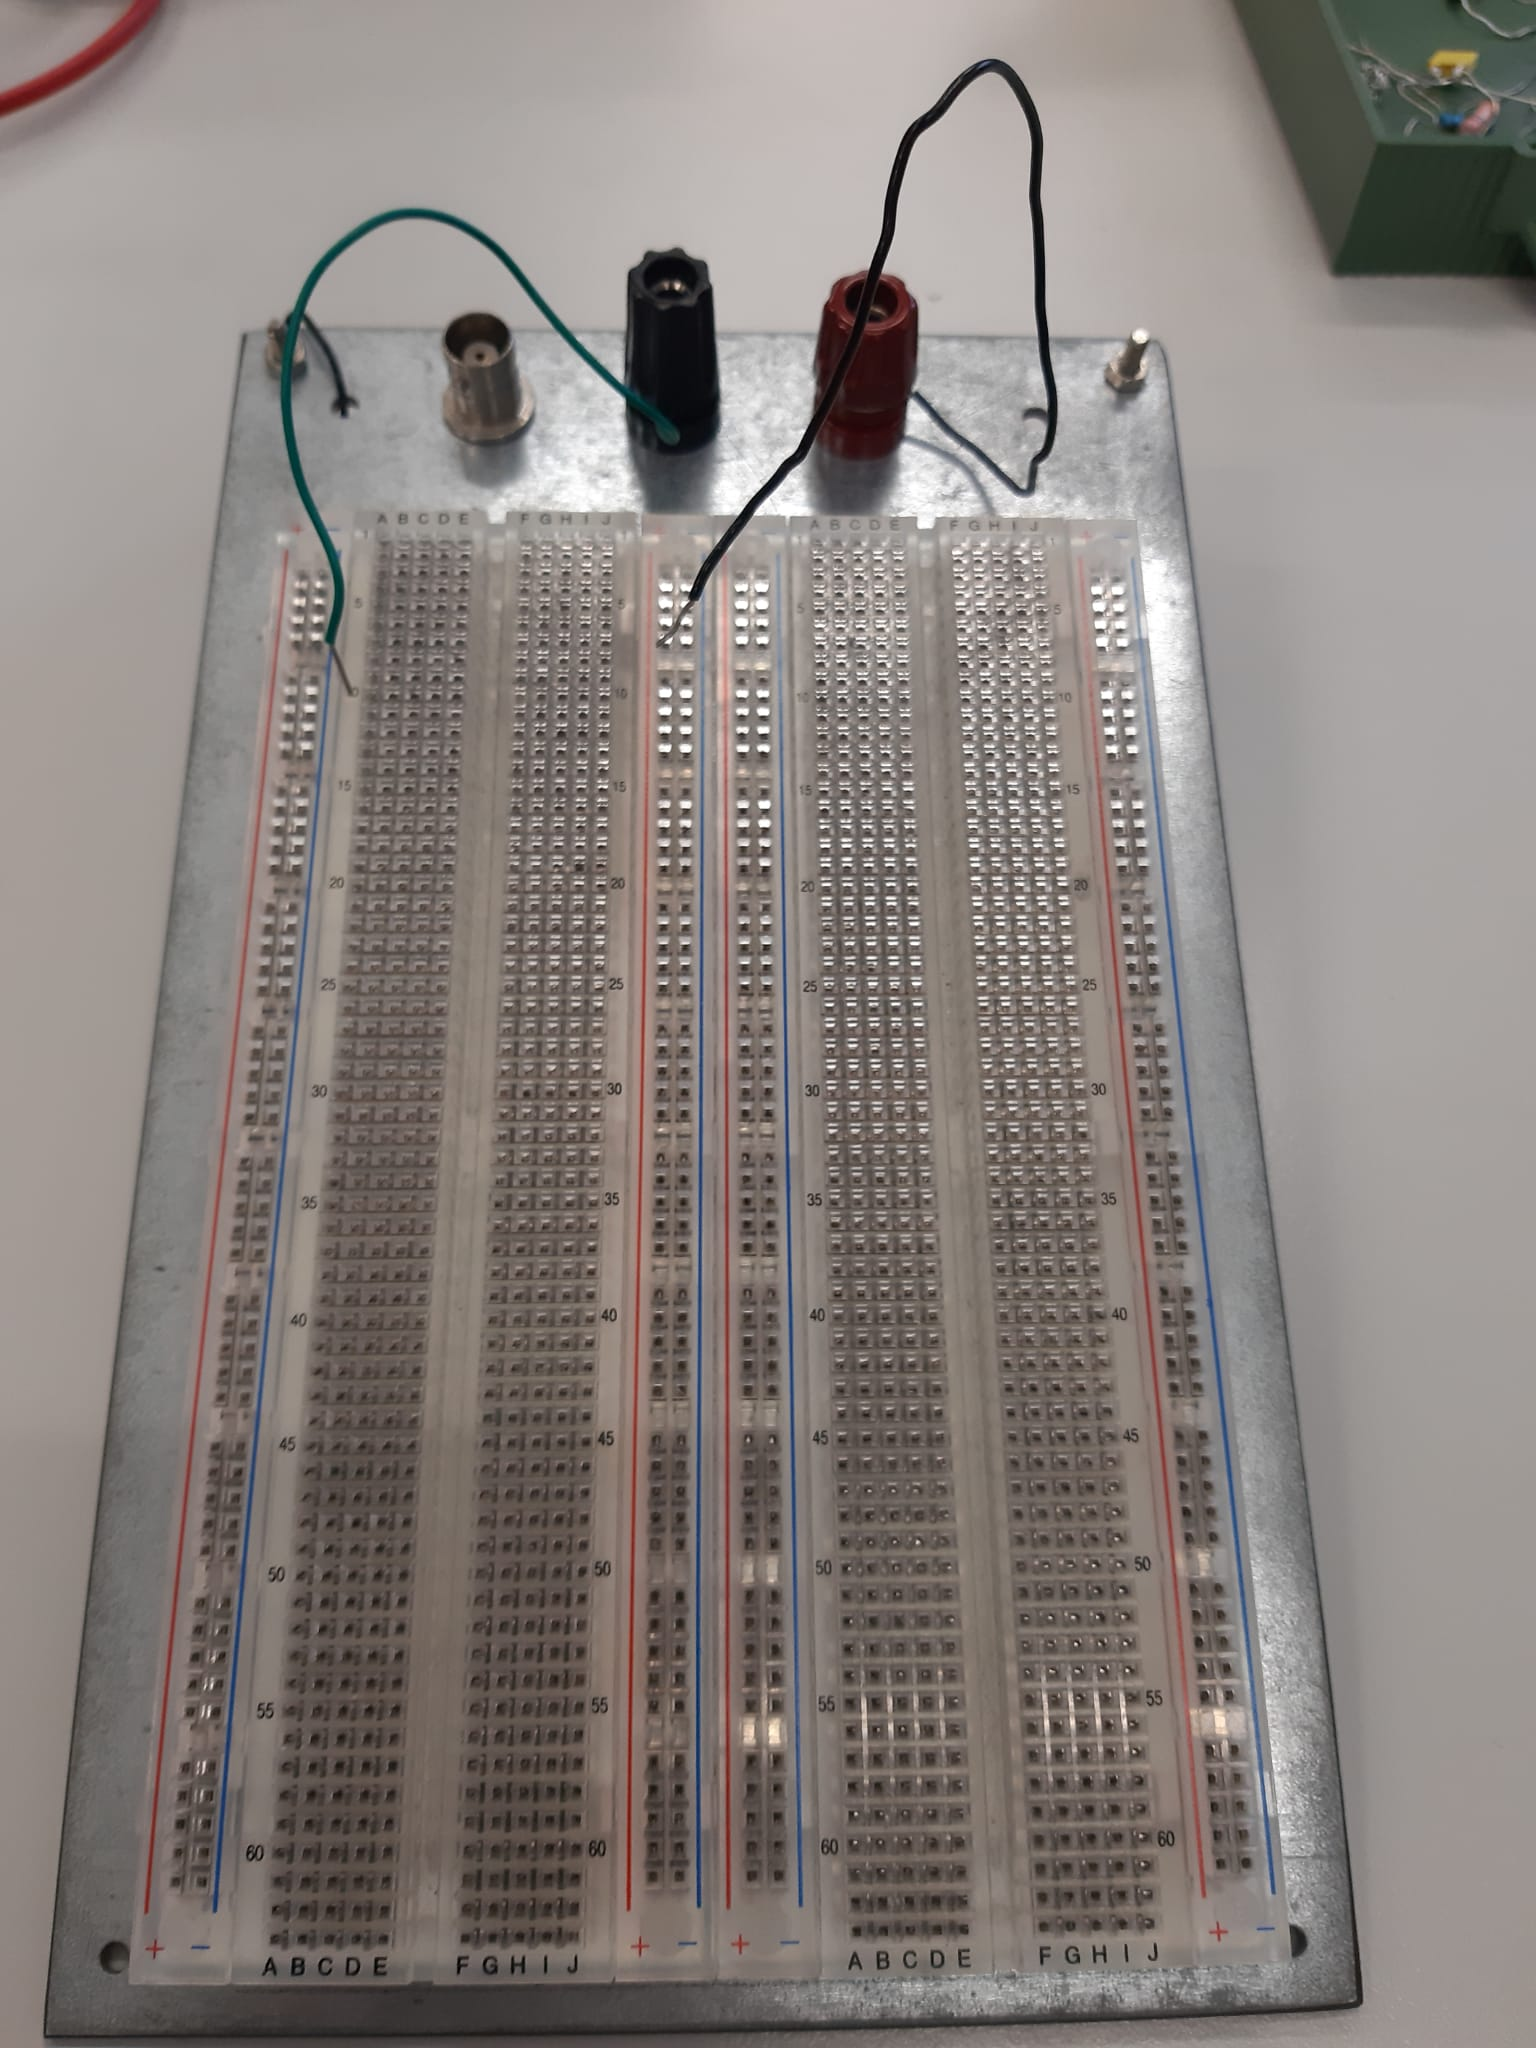
\includegraphics[scale=0.1]{Immagini/Circuitoooo.jpeg}
    \label{fig:my_label}
\end{figure}

La prima parte dell'esperienza si è concentrata sullo studio della strumentazione di laboratorio, studio finalizzato ad utilizzare configurazioni adeguate nelle parti successive. E' stato, infatti, necessario verificare che il multimetro usato come Voltmetro fosse ben progettato, cioè che avesse la caratteristica di possedere una resistenza in parallelo grande. Analogamente, è stato necessario verificare che il multimetro usato come Amperometro avesse la caratteristica di possedere una resistenza in serie piccola.
Successiavmente ci siamo concenrati sullo studio delle resistenze e della Legge di Ohm:

\begin{equation}
\frac{1}{R_{\parallel}}=\sum_{i=1}^{N}\frac{1}{R_{i}} \hspace{73 pt} R_{\perp}=\sum_{i=1}^{N}R_{i}
\end{equation}

\begin{equation}
V=R_{tot}I
\end{equation}

Infine, abbiamo studiato la Legge di Shockley, che descrive l'andamento di corrente per i diodi:

\begin{equation}
I=I_{0}(e^{qv/gK_b T}-1)
\end{equation}

indicando con \textit{q} la carica degli elettroni, con $K_b$ la costante di Boltzmann, con \textit{g} la costante che dipende dal tipo di diodo e con T la temperatura del diodo in Kelvin, corrispondente a quella dell'ambiente. Il termine di proporzionalità $I_0$ è detto \textit{intensità di corrente di saturazione}, il valore che ci aspettiamo di ottenere è molto piccolo in quanto si tratta di una corrente generata dai portatori di carica interni al diodo in diffusione dalla regione neutra alla regione di carica spaziale\footnote{Si tratta di una regione isolante all'interno di un semiconduttore drogato.}.
%% Place large figures that span the whole width of the page in here to easily move them around in the file
% and to avoid getting figures displayed after references and appendix. 
%
% Use {figure*} for a figure that will span both columns. 
% Below is an example of a figure with 6 sub-figures.
\begin{figure*}
%
        \subfigure[Contour plot number 1]{%
            \label{fig:Contour_1}
            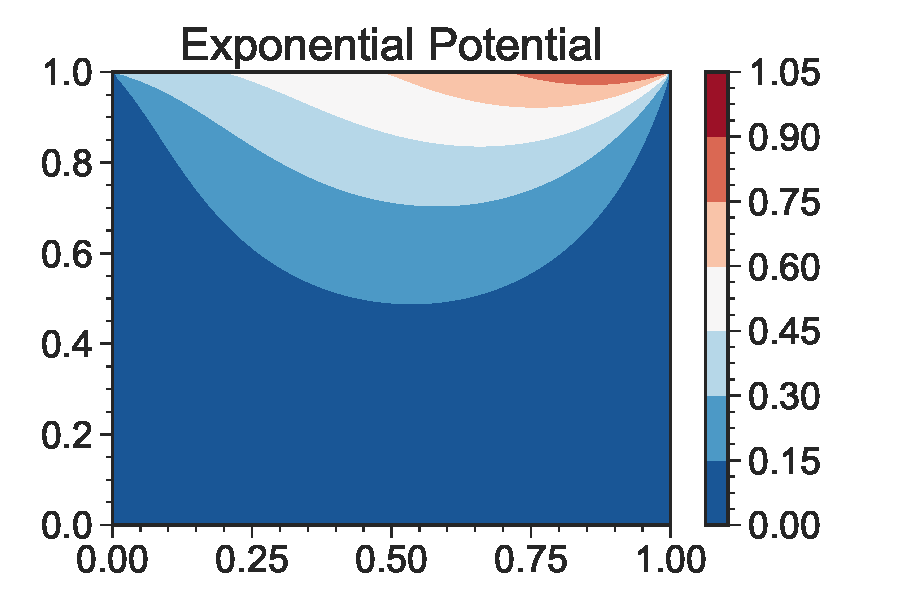
\includegraphics[width=0.3\textwidth]{Images/Fig:Countour-plot/1-contour.pdf}
        }%
        \hspace{1em}
        \subfigure[Contour plot number 2]{%
            \label{fig:Contour_2}
            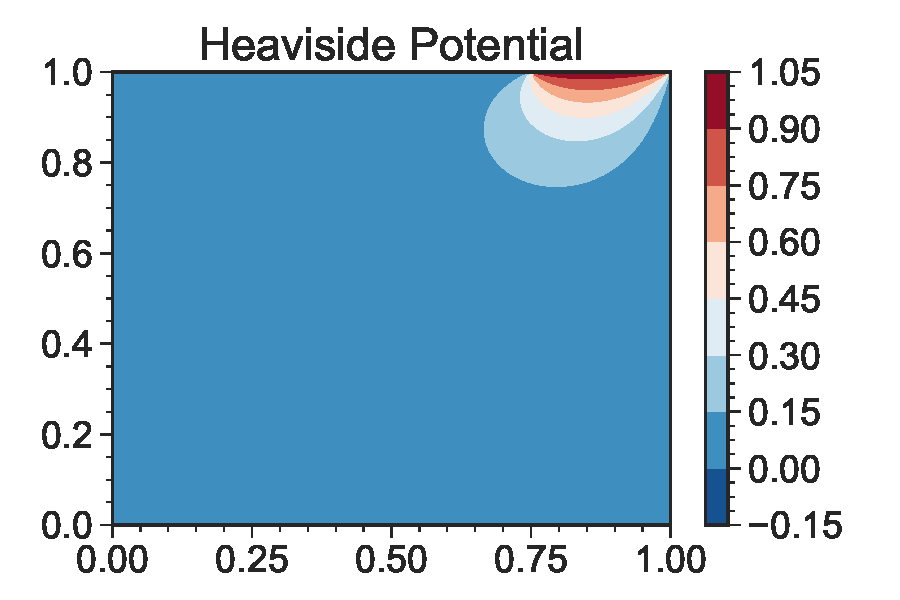
\includegraphics[width=0.3\textwidth]{Images/Fig:Countour-plot/2-contour.pdf}
        }%
        \hspace{1em}
        \subfigure[Contour plot number 3]{%
           \label{fig:Contour_3}
           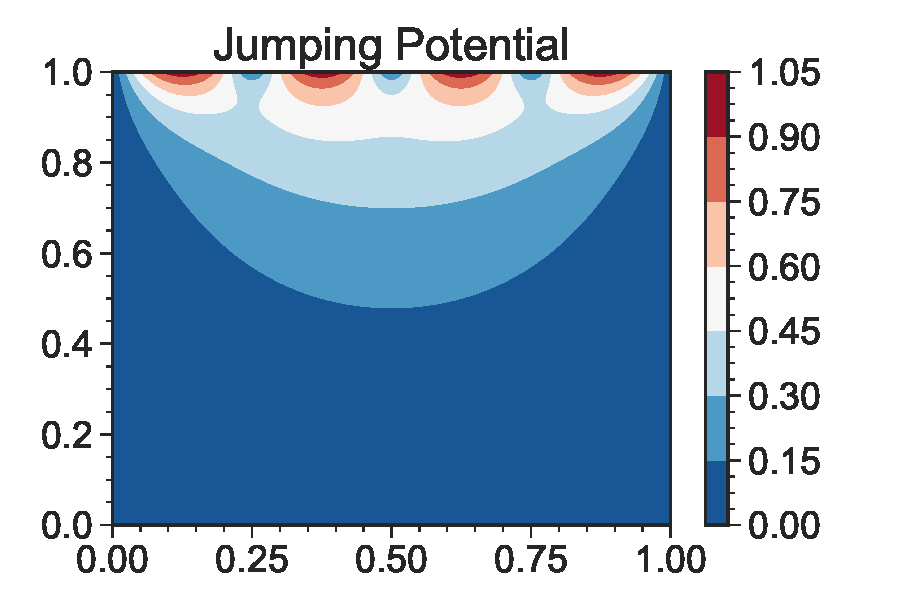
\includegraphics[width=0.3\textwidth]{Images/Fig:Countour-plot/3-contour.pdf}
        }\\ %  ------- End of the first row ----------------------%
        \subfigure[Contour plot number 4]{%
            \label{fig:Contour_4}
            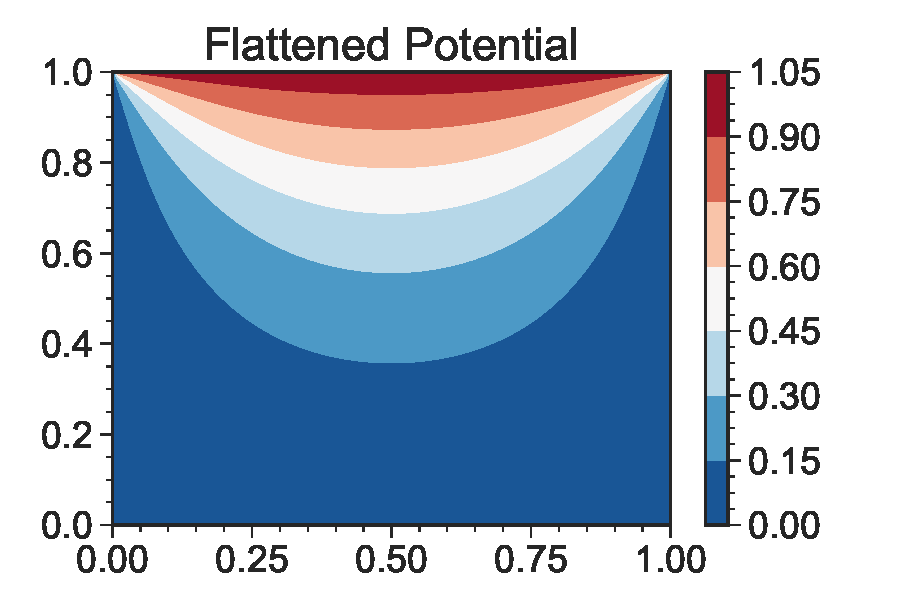
\includegraphics[width=0.3\textwidth]{Images/Fig:Countour-plot/4-contour.pdf}
        }%
        \hspace{1em}
        \subfigure[Contour plot number 5]{%
            \label{fig:Contour_5}
            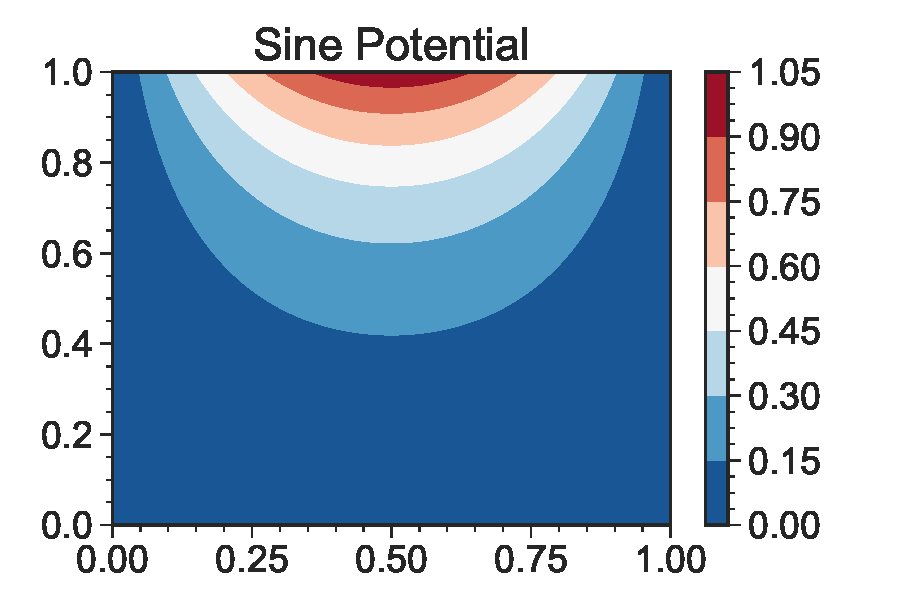
\includegraphics[width=0.3\textwidth]{Images/Fig:Countour-plot/5-contour.pdf}
        }%
        \hspace{1em}
        \subfigure[Contour plot number 6]{%
            \label{fig:Contour_6}
            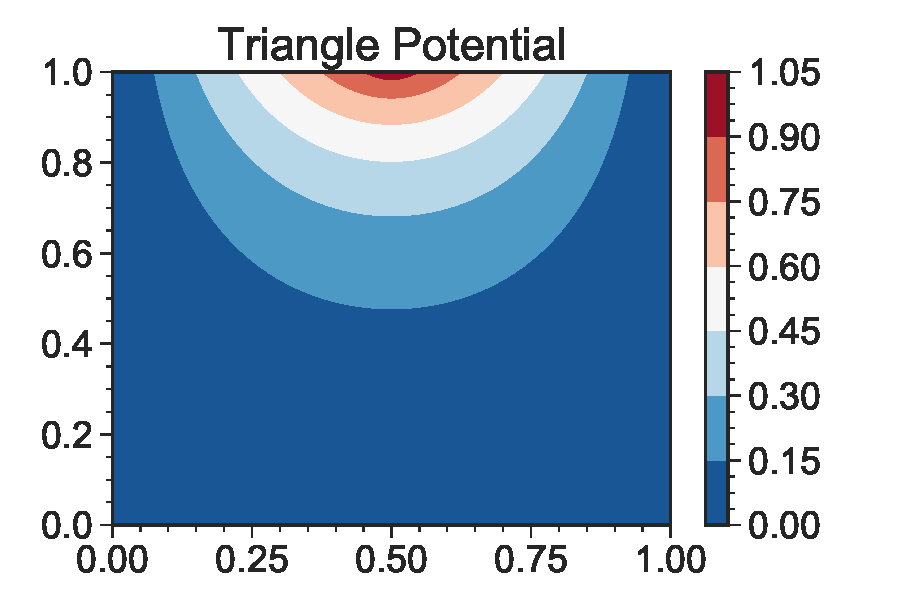
\includegraphics[width=0.3\textwidth]{Images/Fig:Countour-plot/6-contour.pdf}
        }%
%
    \caption{%
        Contour plots for different potentials $V_0(x)$, along the line $y=1$
     }%
   \label{fig:Countour-plot}
\end{figure*}                     % Change this to another line to move big figures.
\section{Circuiti RC e RL}

\begin{figure}[H]
    \centering
    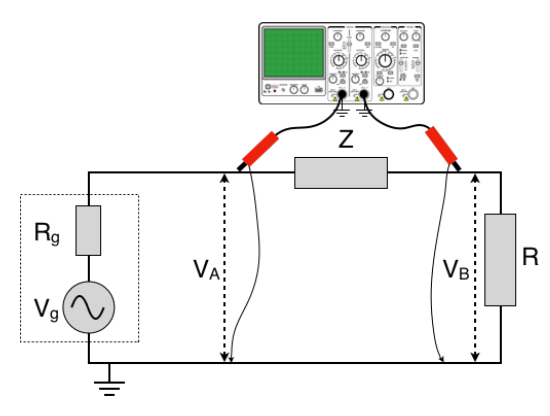
\includegraphics[scale=0.5]{Immagini/RC.PNG}
    \caption{}
\end{figure}


Per entrambe le configurazioni abbiamo disposto il circuito come in figura, dove Z indica rispettivamente il condensatore e l'induttore. Abbiamo, quindi, collegato le sonde come mostrato.
Grazie all'utilizzo dell'oscilloscopio abbiamo misurato diverse grandezze: le ampiezze $V_{A}$ e $V_{B}$ dei due segnali, l'ampiezza $V_{B-A}$ del sgnale differenza $V_{A}(t)$ - $V_{B}(t)$, la differenza di fase $\Delta \phi'$ tra il segnale di tensione ai capi di Z (tra $V_{A}(t)$ - $V_{B}(t)$ e $V_{A}(t)$) e la differenza di fase $\Delta \phi''$ tra $V_{A}(t)$ e $V_{B}(t)$.

Per ciascun circuito abbiamo riportato i dati in una tabella.

\subsection{Circuito RC}
Per svolgere la prima parte dell’esperienza abbiamo raccolto la maggior parte dei dati utilizzando i cursori dell’oscilloscopio, riportandoli successivamente nella seguente tabella; solo le differenze di fase sono state invece calcolate utilizzando i dati presi attraverso l'uso di una chiavetta USB

\begin{table}[!ht]
    \centering
    \begin{tabular}{lllll}
    \toprule
        $\nu$ [Hz]  & $\omega$ & $V_a$ [V] & $V_b$ [V] & $V_{a-b}$ [V]  \\ 
        \midrule
        25  & 3,98  & 2,48 & 0,32 & 2,48  \\ 
        35  & 5,57  & 2,18 & 0,38 & 2,16  \\ 
        45  & 7,16  & 1,92 & 0,42 & 1,88  \\ 
        60  & 9,55  & 1,62 & 0,44 & 1,56  \\ 
        80  & 12,73  & 1,36 & 0,48 & 1,24  \\ 
        90  & 14,32  & 1,24 & 0,5 & 1,16  \\ 
        100  & 15,92  & 3,76 & 1,56 & 3,44  \\ 
        200  & 31,83  & 2,48 & 1,68 & 1,84  \\ 
        300  & 47,75  & 2,21 & 1,68 & 1,28  \\ 
        \bottomrule
    \end{tabular}
    \caption{}
    \label{tabella 1}
\end{table}


Essendo la funzione di trasferimento un numero complesso abbiamo diviso il suo studio nell’analisi del modulo e nell’analisi della fase.
Riportiamo di seguito i moduli della funzione di trasferimento del circuito RC (in cui abbiamo 
usato R = 10$\Omega$), il primo utilizza la differenza di potenziale $V_{a}$ e $V_{b}$ e il secondo $V_{a-b}$ e $V_{b}$.

\begin{figure}[H]
    \centering
    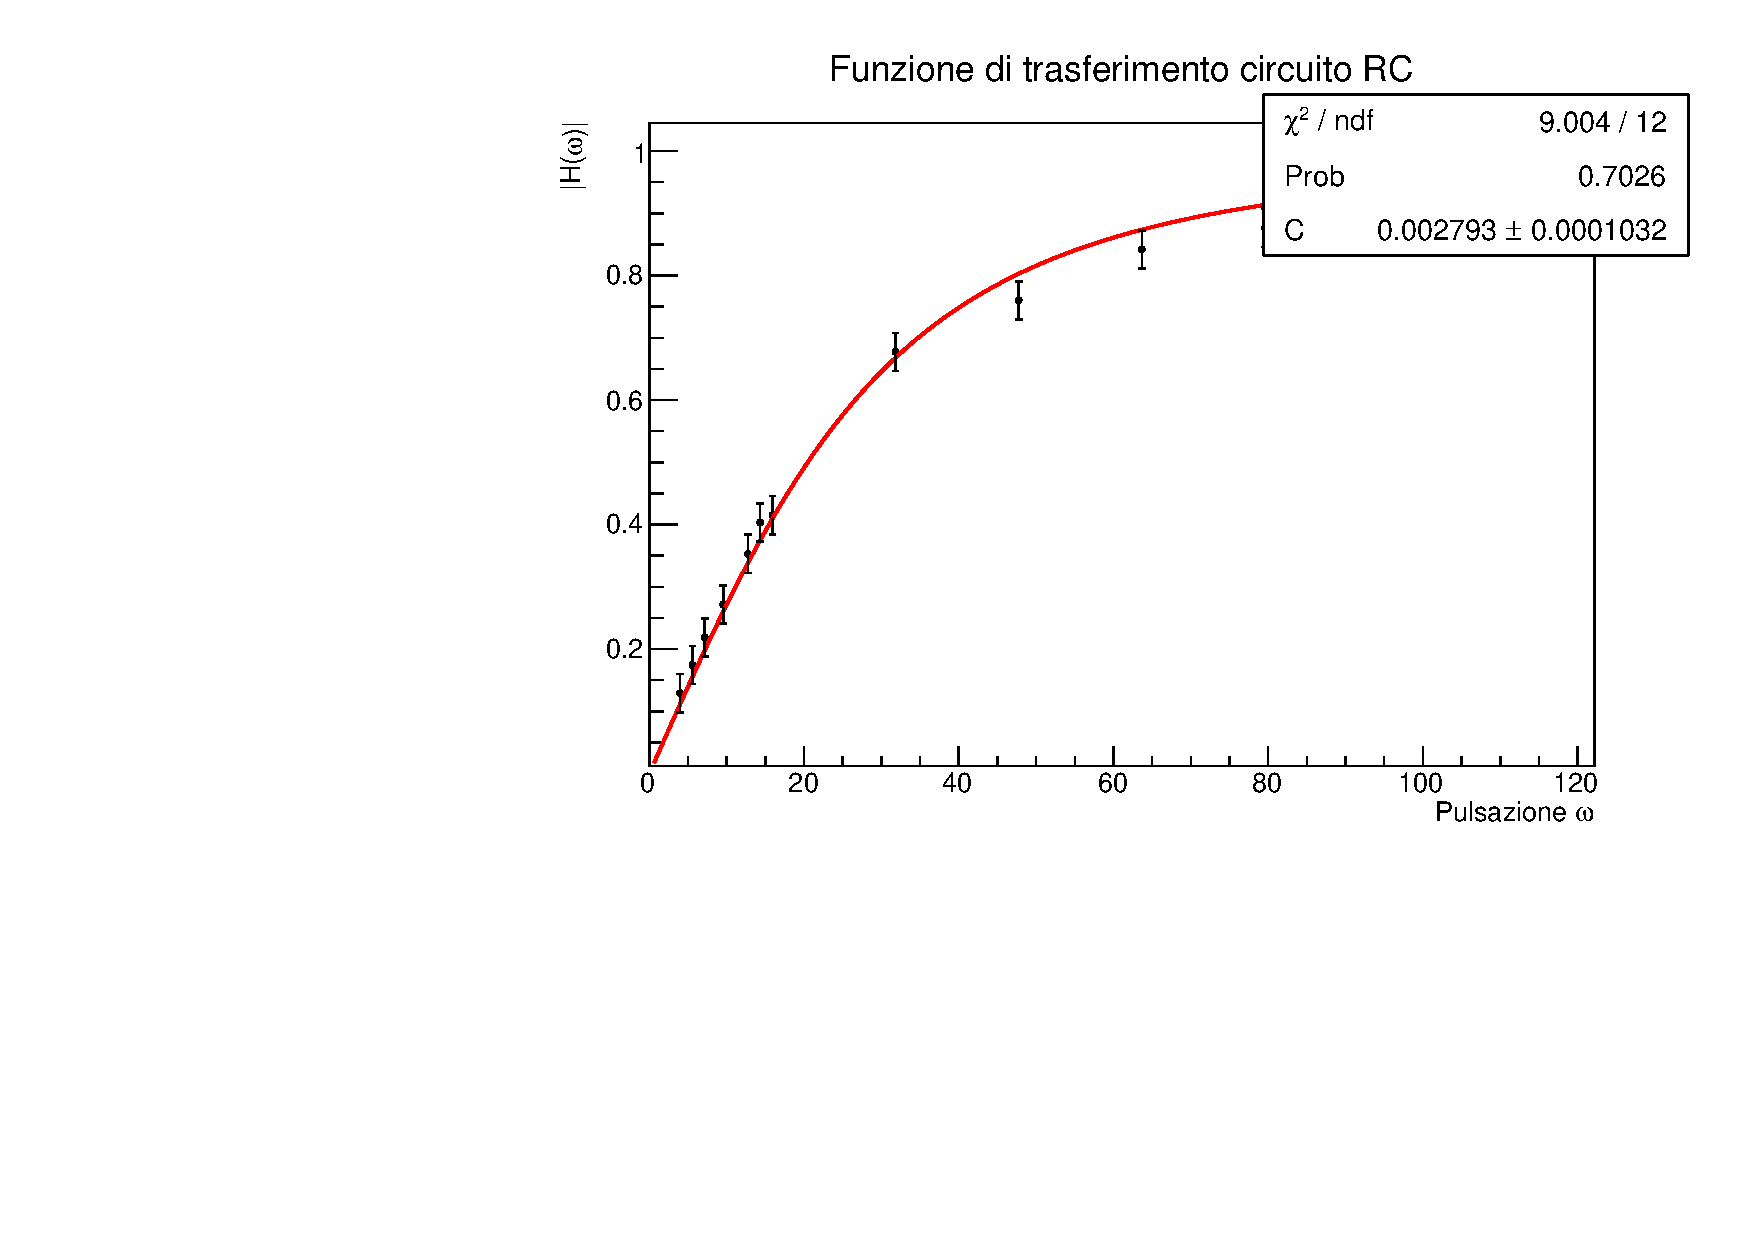
\includegraphics[scale=.4]{Immagini/trasferimento RC.pdf}
    \\
    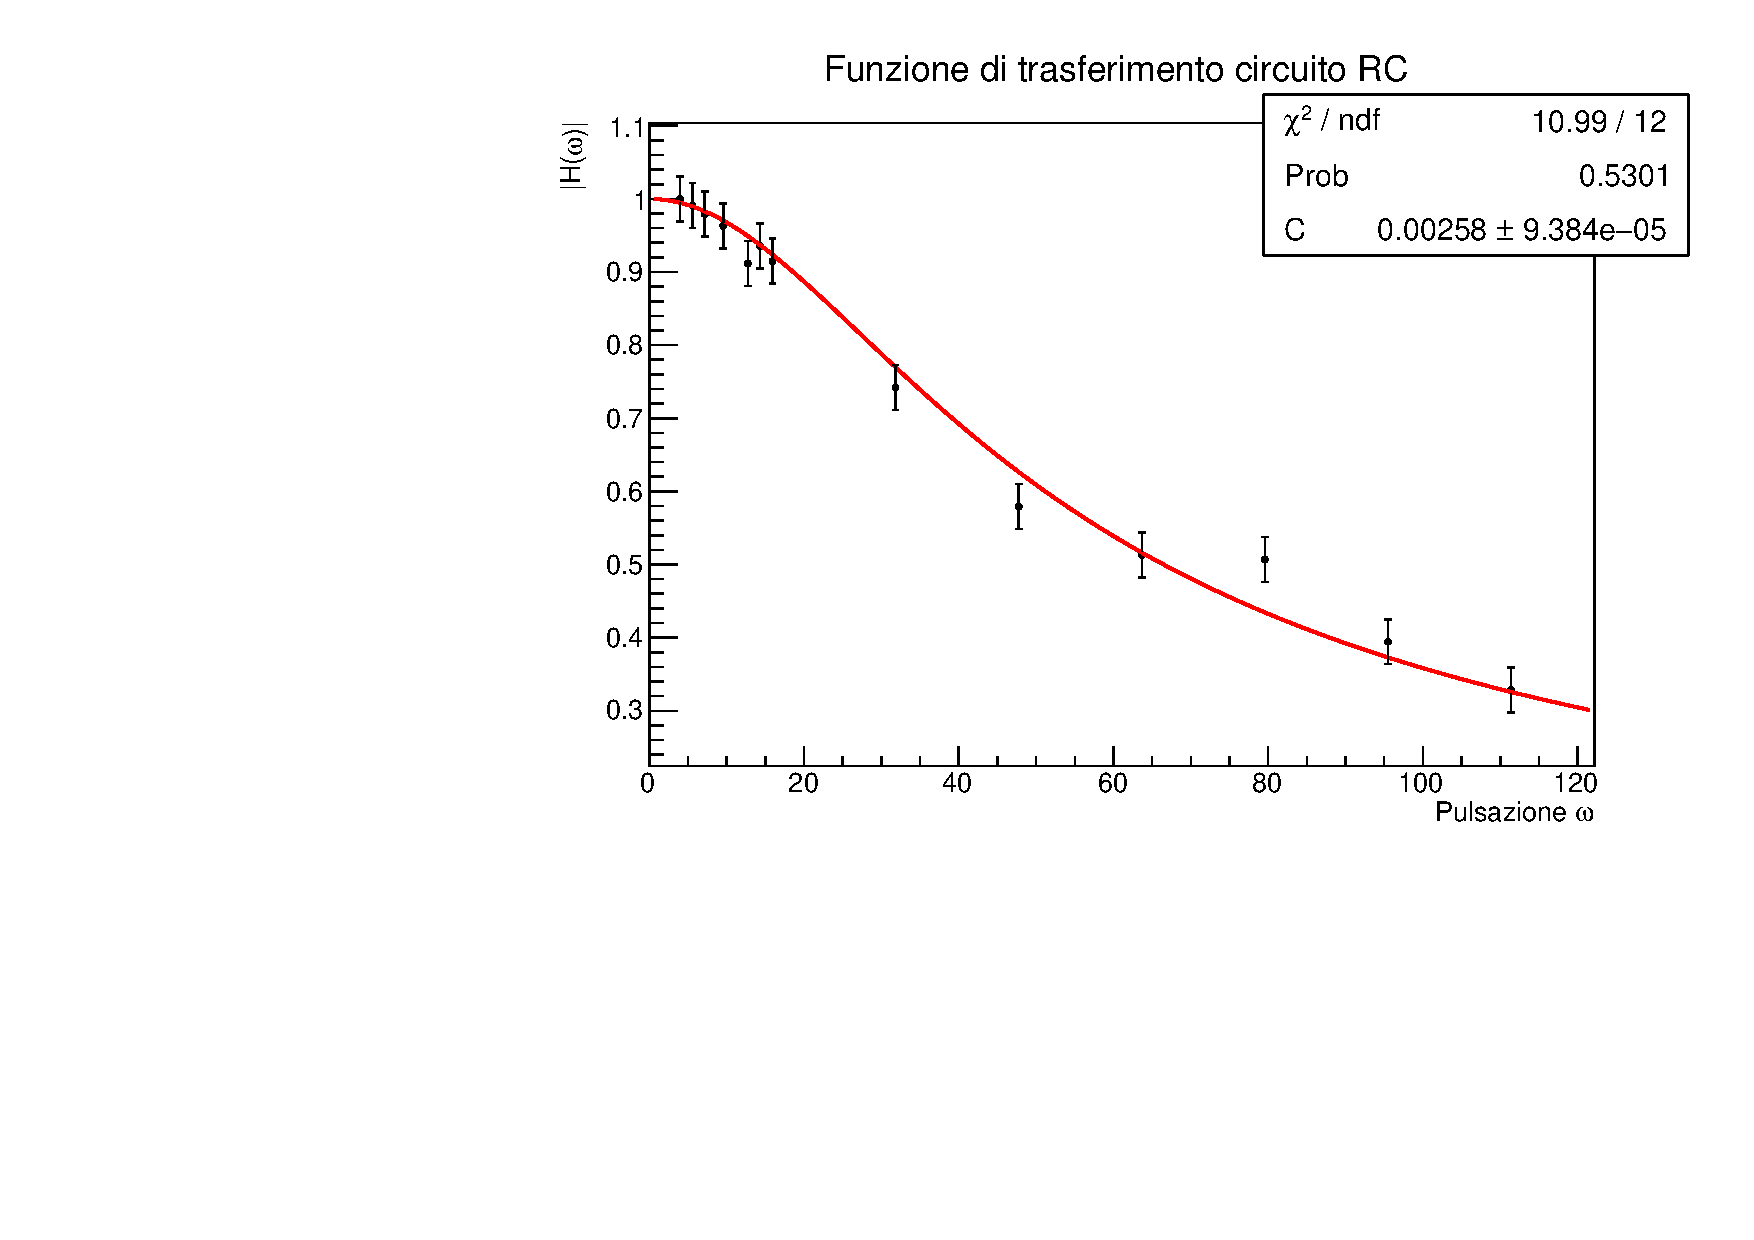
\includegraphics[scale=.4]{Immagini/trasferimento RC 2.pdf}
    \caption{}
\end{figure}

Il parametro \textit{C} corrisponde alla capacità, il suo valore è $(0,0027 \pm 0,0001) F$, inoltre il $\chi ^{2}$ accettabile conferma la relazione aspettata dal modello. Il valore ricavato della capacità è stato ricavato tramite una media pesata con la probabilità di $\chi^2$ dei due valori ricavati dal fit.
La scelta di \textit{R} per costruire il circuito è stata fatta in modo da avere una resistenza \textit{R} molto minore rispetto a quella interna dell’oscilloscopio.


\begin{figure}[H]
    \centering
    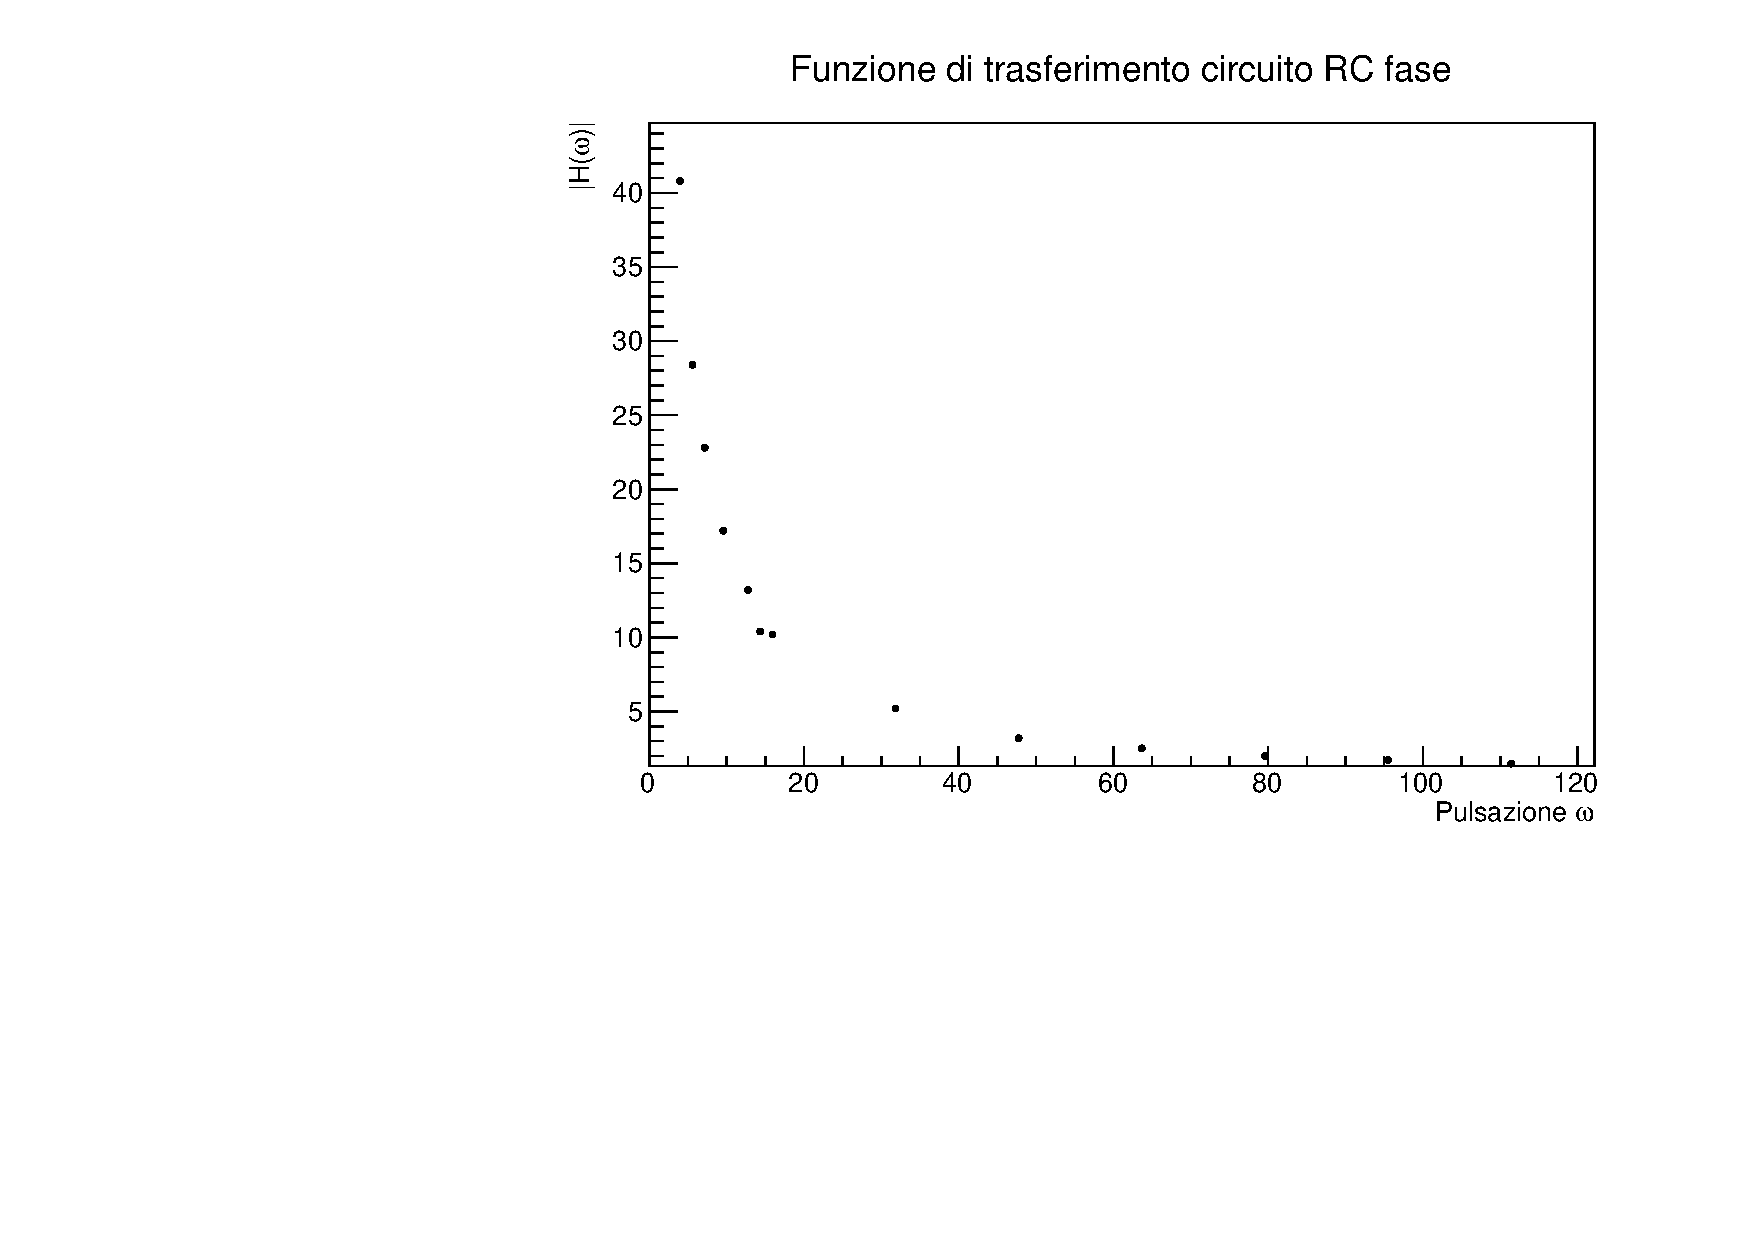
\includegraphics[scale=.4]{Immagini/fase RC.pdf}
    \caption{}
\end{figure}

Come si puo’ evincere dal grafico proposto, i dati raccolti non corrispondono al modello, che dovrebbe seguire un andamento arcotangente.
Le differenze di fase sono state calcolate come differenza 
tra gli zeri per assicurarci miglior precisione. Gli zeri sono stati ottenuti direttamente dall’oscilloscopio attraverso l'uso di una chiavetta USB, in modo tale da poter analizzare un range di 
dati legato alla precisione dello strumento stesso al posto che uno solo. Nonostante i nostri sforzi nel cercare di legare i dati al modello non siamo riusciti nell'intento. Abbiamo ipotizzato che le scale dei tempi fossero sbagliate, abbiamo tentato di calcolare le fasi attraverso le differenze di massimi e di minimi o interpolando l'intero andamento dei segnali per ricavare come parametro le varie fasi, abbiamo provato a lavorare con il modulo della differenza e abbiamo provato ridefinendo la funzione argomento. Nonostante tali accorgimenti non siamo riusciti a individuare una causa di errore attribuibile alla disposizione dei nostri dati rispetto al modello. Tenendo conto delle osservazioni qui riportate siamo costretti a dichiarare il nostro studio sulle fasi invalido.

\subsection{Circuito RL}
Similmente al circuito RC, nel caso di RL (in cui abbiamo utilizzato R = 1k$\Omega $) i moduli della fase di riferimento escono congruenti alla relazione descritta all’interno del modello.
\begin{table}[!ht]
    \centering
    \begin{tabular}{lllll}
    \toprule
        $\nu$ [Hz]  & $\omega$ & $V_a$ [V] & $V_b$ [V] & $V_{a-b}$ [V]  \\ \midrule
        20  & 3,18 & 2,94 & 2,78 & 0,24  \\ 
        50  & 7,96 & 2,94 & 2,76 & 0,28  \\ 
        100  & 15,91 & 2,96 & 2,76 & 0,32  \\
        300  & 47,75 & 2,96 & 2,76 & 0,56  \\
        500  & 79,57 & 3 & 2,72 & 0,88  \\ 
        800  & 127,32 & 2,96 & 2,6 & 1,2  \\ 
        1000  & 159,15 & 2,96 & 2,52 & 1,44  \\ 
        5000  & 795,77 & 3,08 & 1,16 & 2,88  \\
        10000  & 1591,54 & 3,04 & 0,68 & 3,12  \\ \bottomrule
    \end{tabular}
    \label{tabella 2}
    \caption{}
\end{table}

\begin{figure}[H]
    \centering
    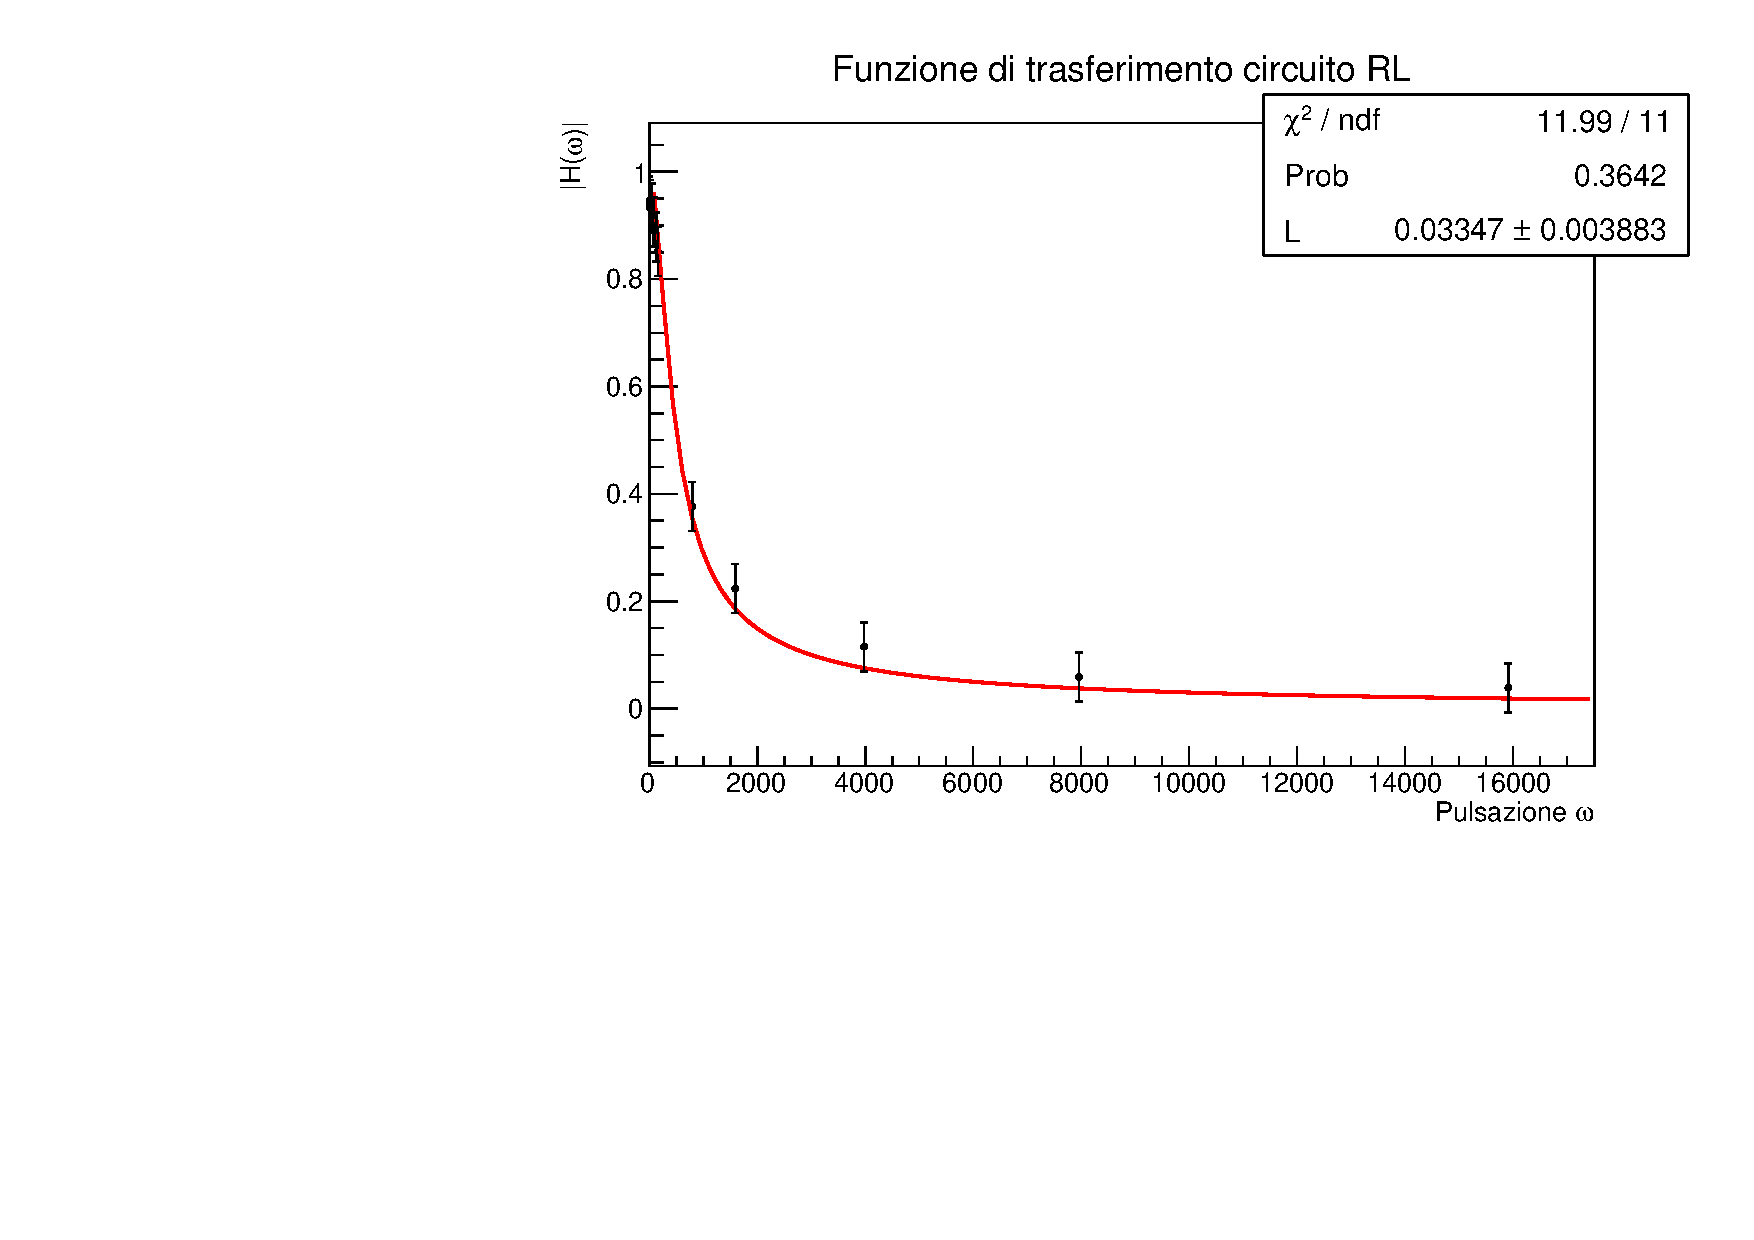
\includegraphics[scale=.4]{Immagini/trasferimento RL.pdf}
    \\
    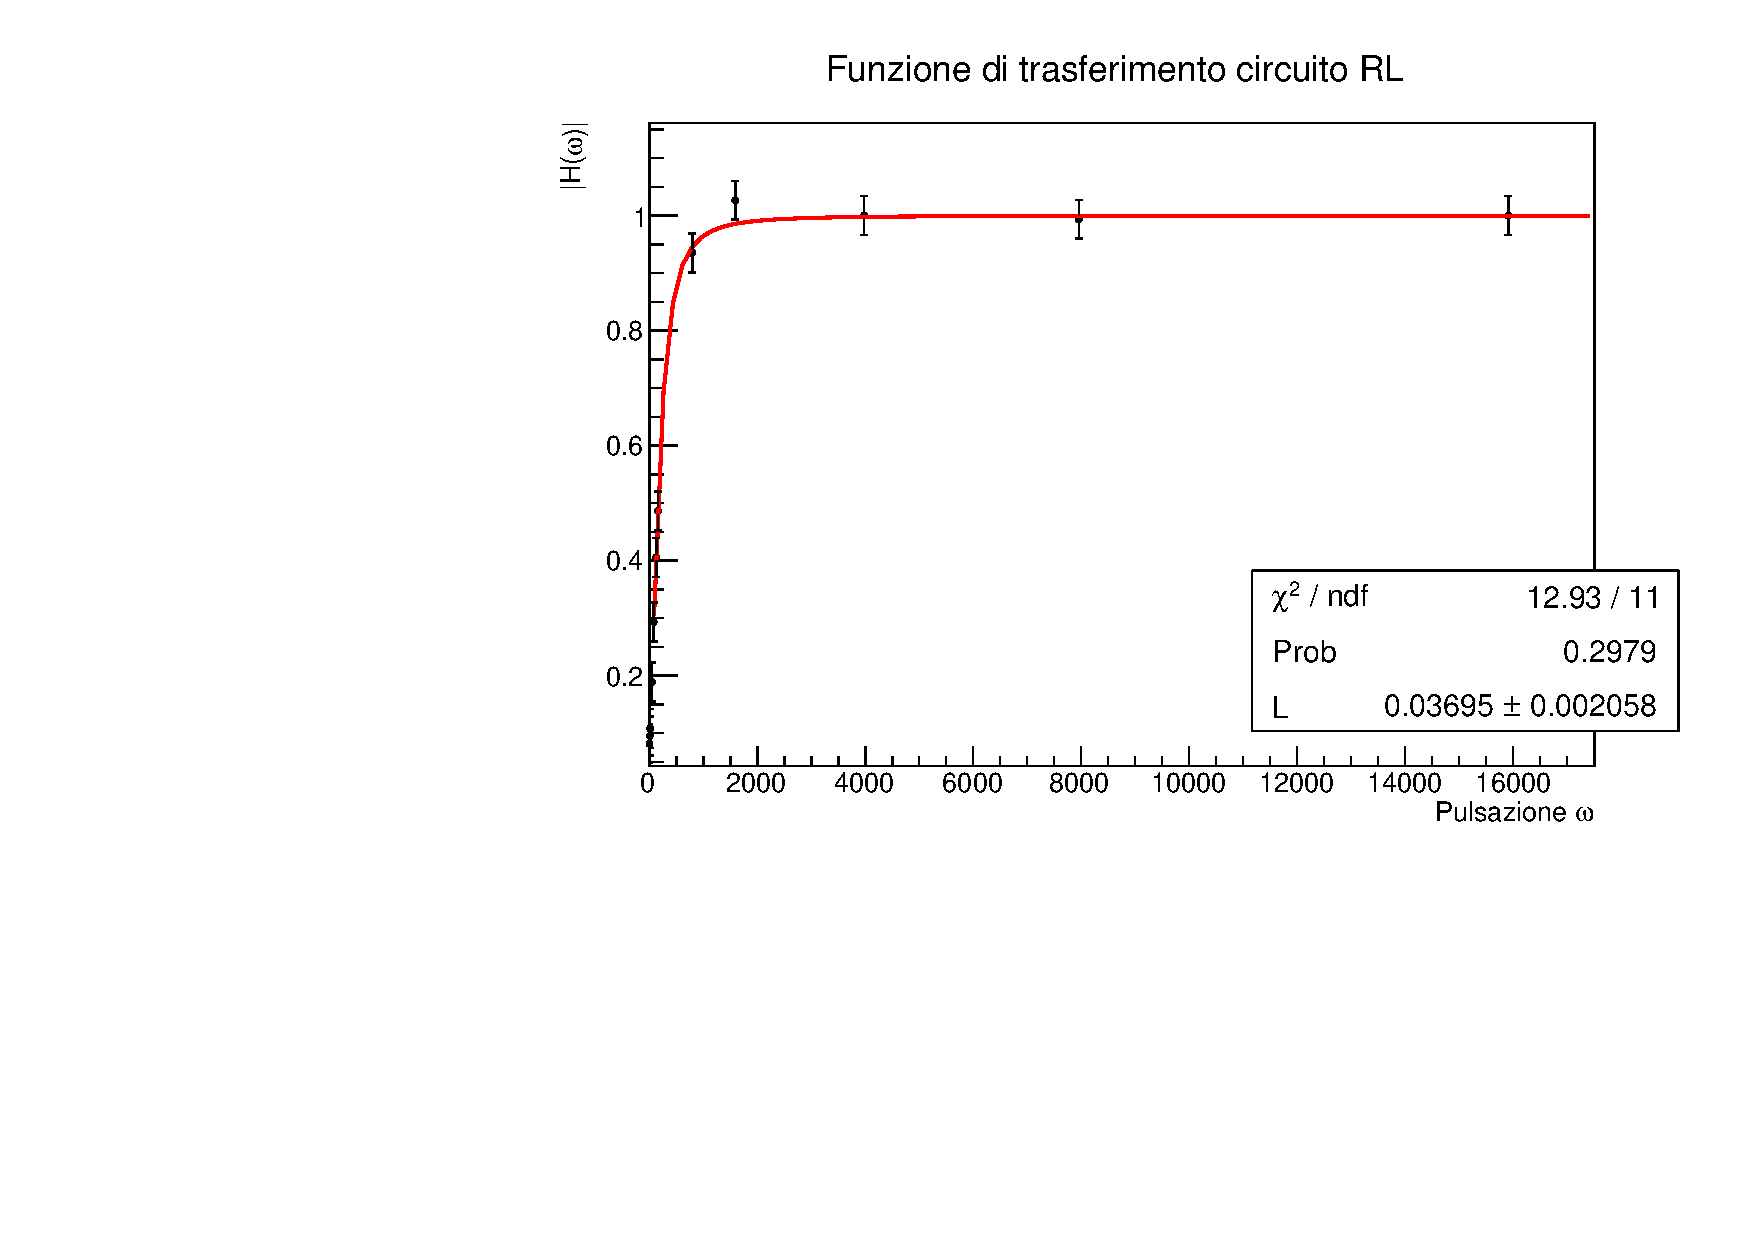
\includegraphics[scale=.4]{Immagini/trasferimento RL 2.pdf}
    \caption{}
\end{figure}

Abbiamo ricavato il valore di $\textit{L}=(0,0346 \pm 0,0001)H$, che corrisponde all’induttanza, ma per le fasi siamo incappati nello stesso problema che avevamo riscontrato per il circuito RC e che rende invalido  il nostro studio delle fasi. 
Il valore di L risulta accettabile in quanto nell’ordine della decina di \textit{mH}.

\section{Circuito RLC}
\begin{figure}[H]
    \centering
    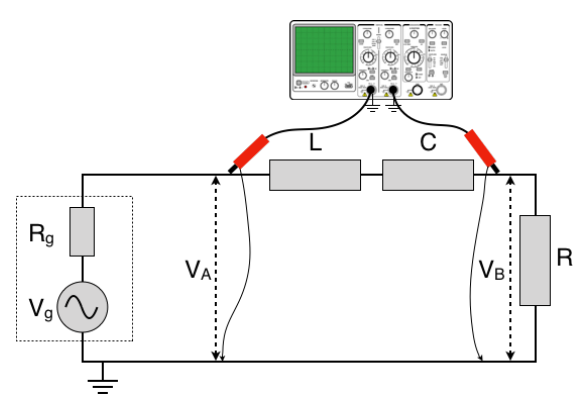
\includegraphics[scale=0.5]{Immagini/RLC.PNG}
    \caption{}
\end{figure}

Abbiamo arrangiato il circuito come in figura servendoci di una resistenza R = 1k$\Omega$.
L’obbiettivo della seconda parte dell’esperimento, similmente a prima, era lo studio della funzione di trasferimento e, attraverso il fit delle funzioni stesse, ricavare i valori dei parametri L e C.
Come in precedenza, abbiamo diviso lo studio suddividendolo in analisi del modulo e analisi della fase. 

\begin{table}[!ht]
    \centering
    \begin{tabular}{lllll}
    \toprule
         $\nu$ [Hz]  & $\omega$ & $V_a$ [V] & $V_b$ [V] & $V_{a-b}$ [V]  \\ 
         \midrule
        5  & 0,80 & 3,04 & 2,6 & 1,2  \\ 
        15  & 2,39 & 3 & 2,76 & 0,48  \\ 
        25  & 3,98 & 3,08 & 2,8 & 0,4  \\ 
        30  & 4,77 & 3,04 & 2,8 & 0,4  \\ 
        35  & 5,57 & 3 & 2,8 & 0,4  \\ 
        45  & 7,16 & 3,04 & 2,8 & 0,32  \\ 
        60  & 9,55 & 3,08 & 2,4 & 0,4  \\ 
        80  & 12,73 & 3,04 & 2,8 & 0,32  \\ 
        100  & 15,92 & 3,04 & 2,8 & 0,32  \\ 
        \bottomrule
    \end{tabular}
    \label{tabella 3}
\end{table}

Riportiamo di seguito i fit relativi ai moduli:

\begin{figure}[H]
    \centering
    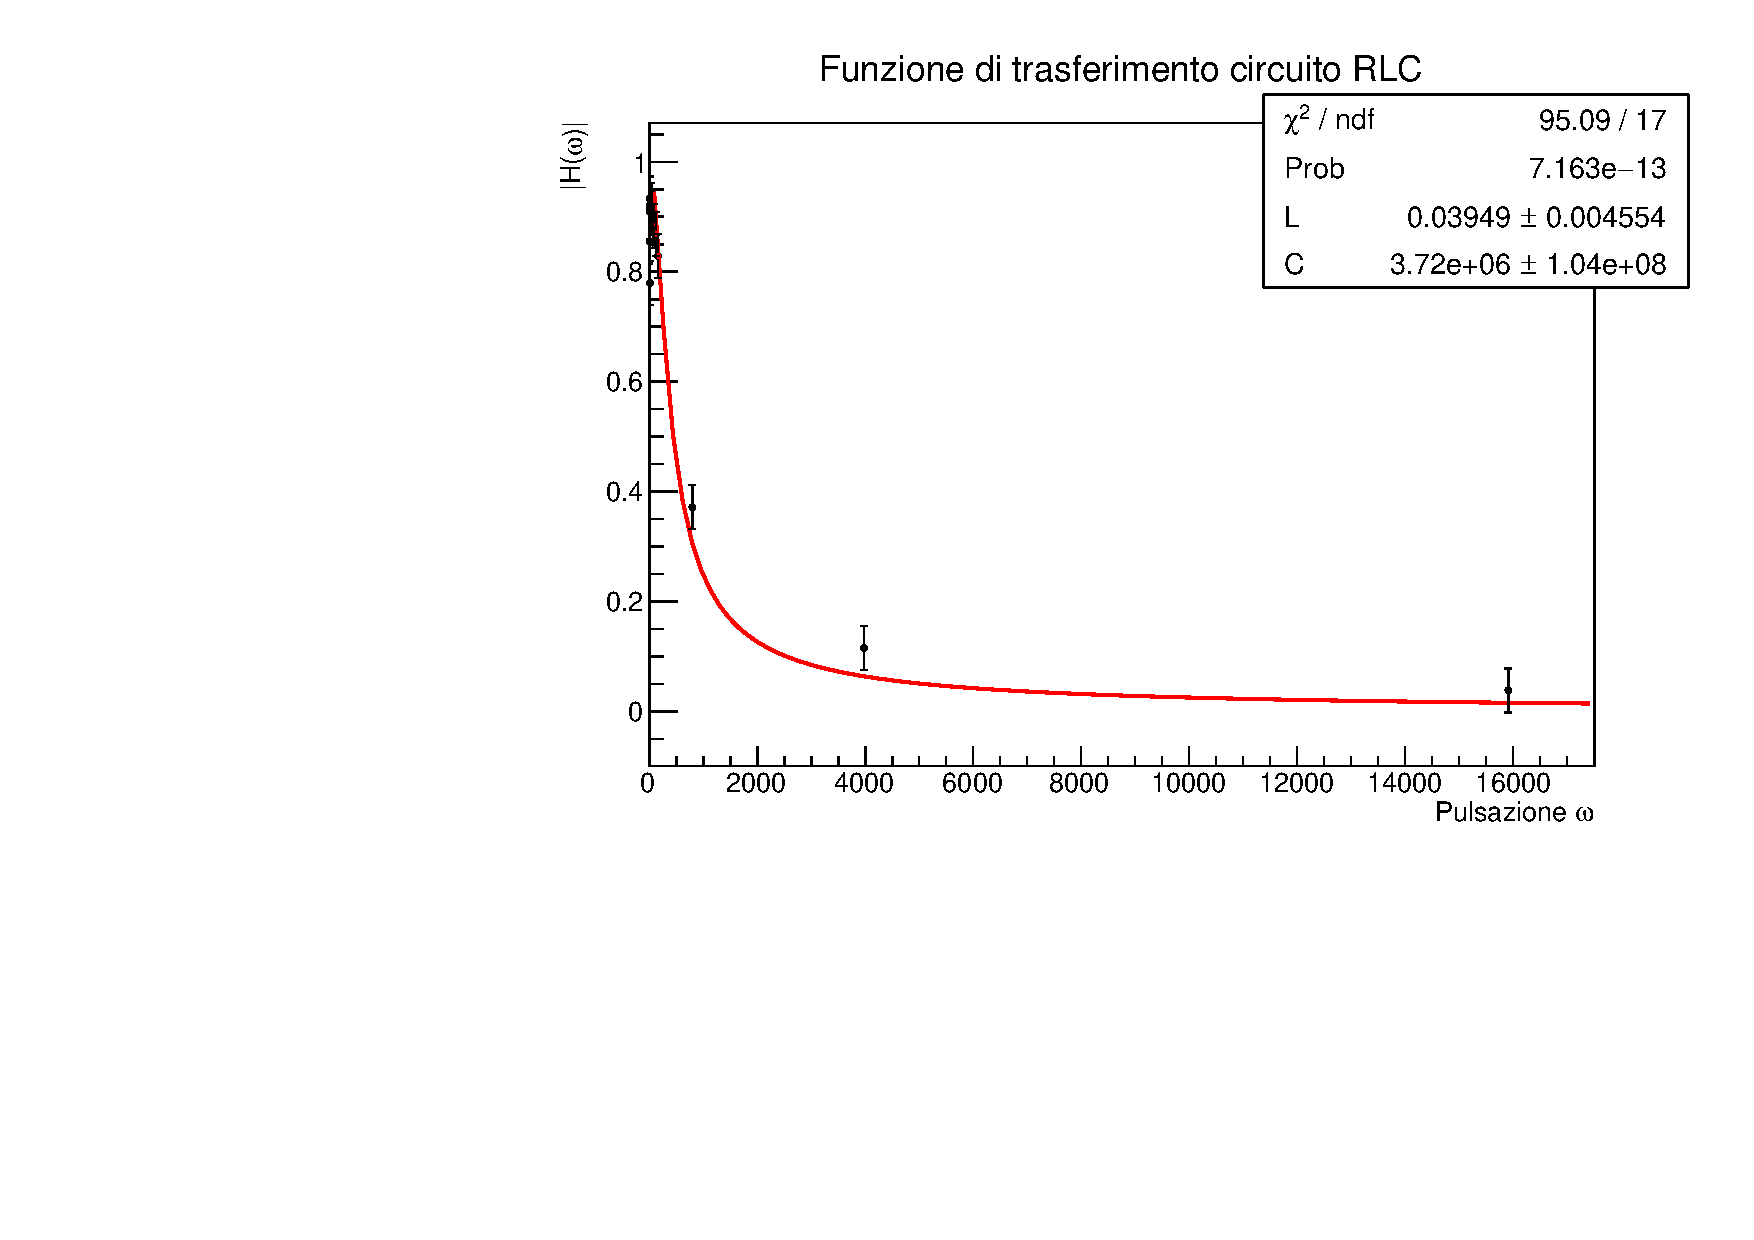
\includegraphics[scale=.4]{Immagini/trasferimento RLC.pdf}
    \\
    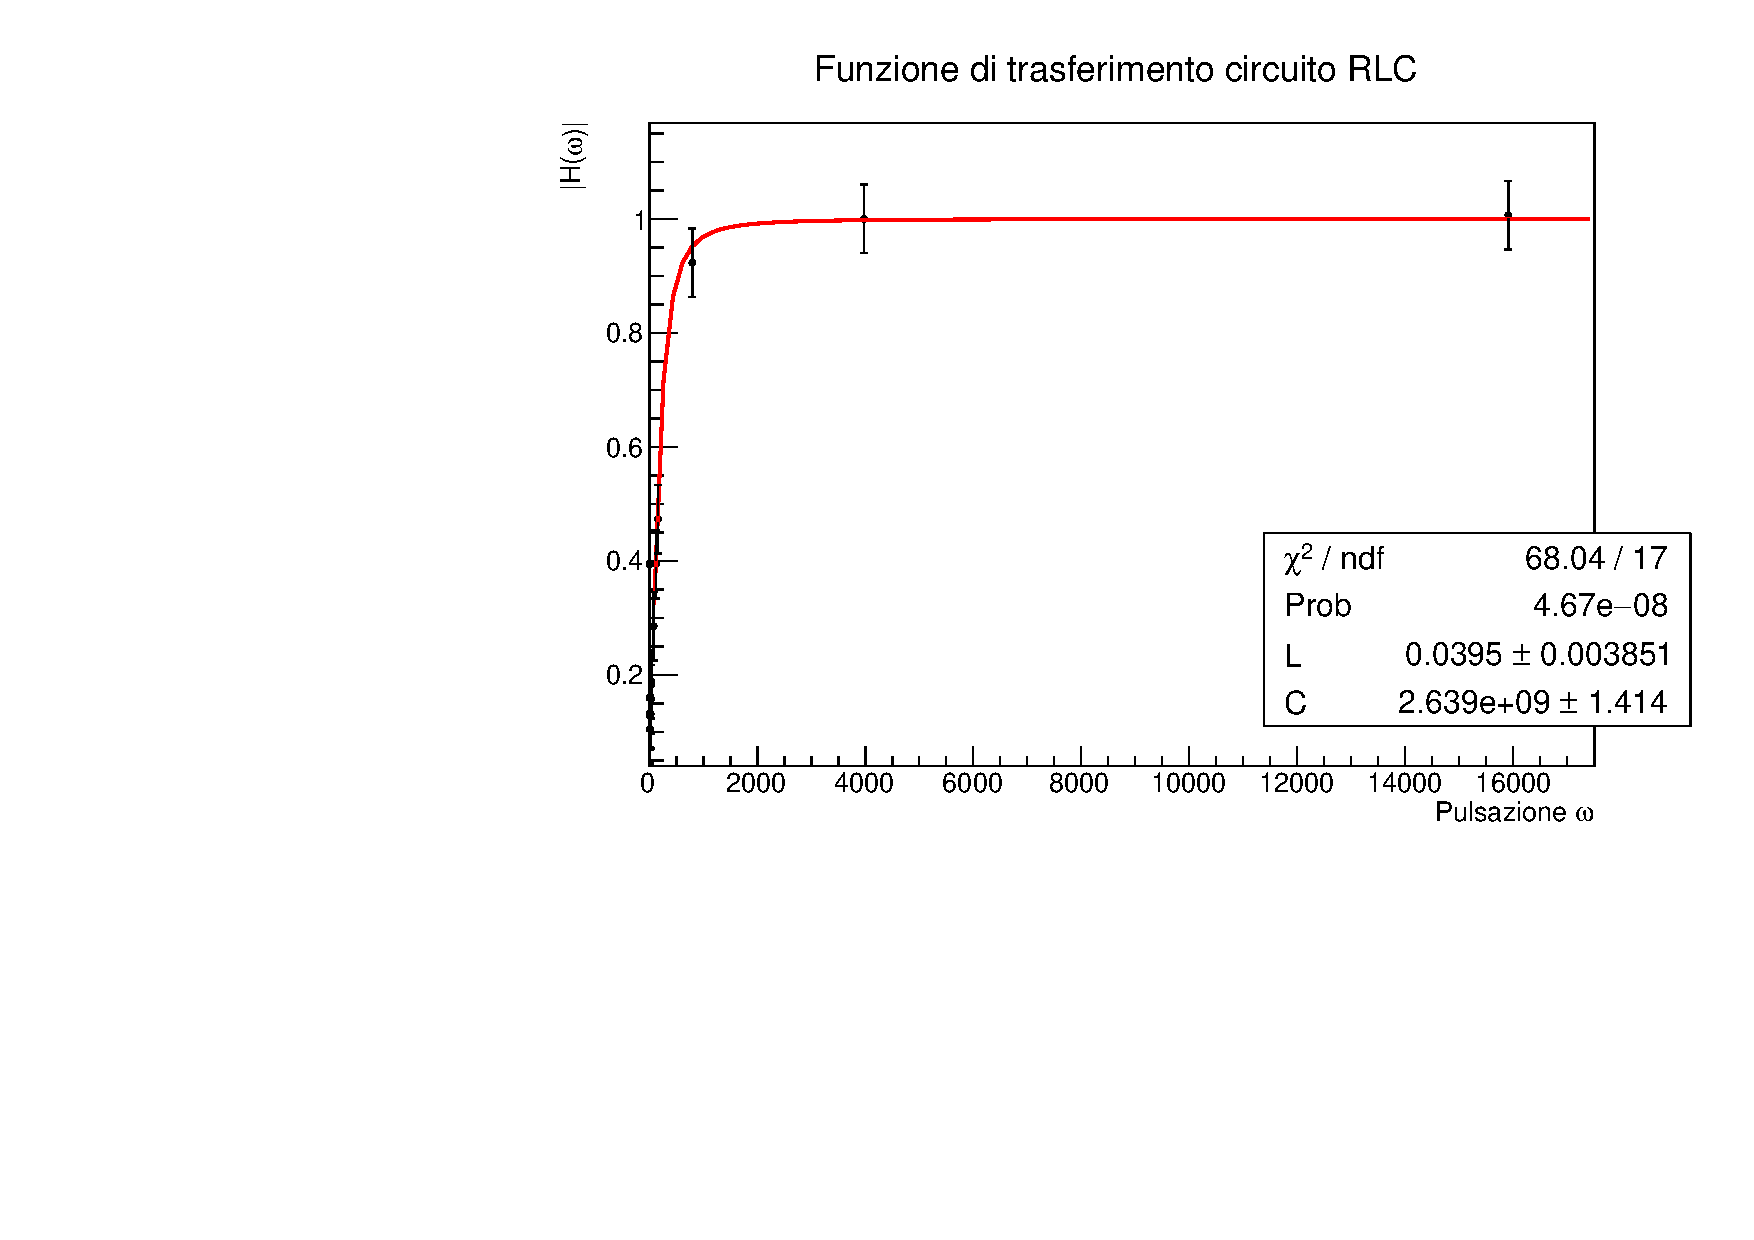
\includegraphics[scale=.4]{Immagini/trasferimento RLC 2.pdf}
    \caption{}
\end{figure}

Com'è possibile osservare dai fit presentati, i dati presentano un $\chi ^{2}$ che indica un’incompatibilità tra modello e misure raccolte, ma fornisce stime sui parametri possibili,
accettabili, in quanto dell’ordine di grandezza aspettato (decine di mHerny per l’induzione e nell’ordine dei $\mu$Farad per la capacità).

I valori di C ed L sono riportati nei grafici.

Riteniamo che il modello non venga verificato, non a causa delle misure raccolte o a causa di errori nel modello, ma a causa di un possibile mal funzionamento nell’algoritmo usato per il fit di cui non riusciamo a venire a capo. Il fit, infatti, dovrebbe riportare una funzione a campana, ma, poiché essa presenta il massimo per frequenze molto basse, anche campionando con maggior frequenza in un intorno del massimo stesso è impossibile evidenziare una crescita di ripidità comparabile con la decrescita della funzione stessa. Anche rimuovendo dei punti all’estremità destra della funzione, la crescita rimane troppo 
piccola rispetto alla decrescita e viene evidenziata, inoltre, l’oscillazione del valore del modulo della funzione di trasferimento attorno alla $\Omega$ massima portando quindi il fit a presentare incompatibilità tra modello e misure raccolte.

Come nei casi precedenti lo studio sulla fase non risulta valido.

\section{Discussione errori}
\label{discussione errori}
L'errore associato ad ogni misura è stato generato tramite un algoritmo per la generazione di numeri pseudocasuali. Infatti, eseguendo una misura del segnale senza elementi circuitali inseriti, si osserva che è sempre presente un segnale di disturbo che quindi va ad intaccare ogni misurazione variando l'intensità del segnale misurato.

Siccome è presente in ogni misurazione abbiamo ritenuto plausibile considerarlo come la principale fonte di errore, inoltre a questa fonte si deve aggiungere l'errore sistematico intrinseco dello strumento. Tale errore è stato valutato come la sensibilità dello strumento. Un ulteriore elemento a favore di questa ipotesi è che le misure sono state raccolte direttamente dallo strumento tramite una chiavetta USB per cui, a meno di errori dovuti a malfunzionamenti interni della strumentazione impossibili da identificare, possibili fonti esterne di errore sono da scartare. 

Analizzando il segnale di disturbo si è notata la presenza di valori misurati di tensione distribuiti in maniera casuale. Per tale ragione si è utilizzato un algoritmo di generazione di numeri pseudocasuali distribuiti secondo una \textit{pdf} gaussiana.

La scelta della \textit{pdf} è motivata dal fatto che i valori di tensione osservati erano meno densi agli estremi dell'intervallo mentre la densità aumentava gradualmente spostandosi nel centro dello stesso.


\section{Conclusioni}
Lo scopo di questa esperienza è stato quello di studiare e verficare relazioni e leggi riguardanti resistenze e diodi. In primo luogo è stata condotta una verifica sulle due configurazioni, quella con il voltmetro e quella con l'amperometro, al fine di analizzare i loro comportamenti rispetto alle configurazioni ideali. Per l'amperometro i risultati ottenuti risultano congruenti con quelli aspettati, cosa che invece non accade con il voltmetro. Crediamo che la causa di ciò possa essere dovuta a due principali fattori. In primis riteniamo possibile che la resistenza scelta, la quale era necessario fosse confrontabile con quella del voltmetro, potrebbe non essere stata tale e che, quindi, l'errore sull'ordine di grandezza potrebbe essere stato causato da quello. Come seconda fonte di errore riconduciamo il fatto che, per identificare le resistenze, ci siamo serviti del tool online menzionato nell'introduzione, i cui valori potrebbero non corrispondere a quelli reali, inserendo quindi un possibile errore sistematico nei nostri risultati. A causa di tale incongruenza, in esperienze che fornivano la possibilità di scegliere la configurazione, abbiamo sempre preferito utilizzare quella con l'amperometro. Lo studio sulla relazione evidenziata da Ohm risulta corretta, nonostante il $\chi^2$ risulti molto bassa. La causa più probabile di questo fenomeno potrebbe essere ricercata in una sottostima degli errori, dovuta al nostro modo di identificare i valori delle resistenze. Nonostante questa possibile fonte di errore, lo studio sul partitore resistivo ha portato risultati congruenti rispetto al nostro studio teorico riguardo alle relazioni sulle resistenze. Infine, anche l'analisi sul diodo risulta congruente rispetto alla relazione ipotizzata, con un $\chi^2$ ridotto di circa 0.82. Riteniamo che l'esperimento potrebbe essere riprodotto con risultati più soddisfacenti se si procedesse a misurare le resistenze in maniera differente. 
%\clearpage                                     % Sometimes you want the rest on separate pages.
                % Comment out to exclude the Acknowledgements section

%%%%%%%%%%%%%%%%%%%%%%%%%%%%%%%%%%%%%%%%

% Bibliography
%--------------------


\clearpage                                     % Sometimes it is useful to have appendix on separate page.
%\onecolumn                                     % If you want 1 column for appendix.
\appendix
% Delete the text and write Appendix here (not required, can be omitted):
% Comment out ' \appendix
% Delete the text and write Appendix here (not required, can be omitted):
% Comment out ' \appendix
% Delete the text and write Appendix here (not required, can be omitted):
% Comment out ' \input{Text/Appendix} ' to remove this section.
%------------------------------------
 ' to remove this section.
%------------------------------------
 ' to remove this section.
%------------------------------------
                           % Comment out to exclude appendix

\end{document}

% Notes on Copyright:
%--------------------

% Feel free to use this template as you like.
% I do not require users to give me credit for
% the use of this template, unless you share
% a verbatim (word for word) LaTeX code copy
% on the internet.

% The author may or may not release a new 
% update/ new version of this template.